%************************************************
\chapter{Introducing Simulation}
\label{chapter:introducing_simulation}
%************************************************

\section{The End of the Model}

My description of the model of mind in plain non-technical English is
now complete.  The rest of this part will extend the model that I have
completed describing in English into the assumptions of simulation
that I will need for beginning a mathematical description in
\autoref{part:simulation}.

There is a difference between a model of mind and a simulation of a
model of mind.  I have presented my model of mind in plain English in
the first part of this dissertation.  Simulating the model does not
change the model.  At this point, I am assuming that I have
communicated my model in an understandable way.  I will now augment
this understanding with a separate auxiliary understanding of how to
simulate it.  It is important to explain how the model can be
simulated, so that I can subsequently quantify metrics for evaluation.
Further, understanding how to simulate the model is imperative to
understanding the computational implementation.

\section{Simulation Model}

I will use the term \emph{simulation model} to refer to the model that
changes during the activity of simulation.  It is imperative to
understand that the simulation model is not the same as the model that
I have previously described.  The model of mind does not change in
this dissertation.  The simulation model is an arrangement of symbols
that can be manipulated in order to simulate the model of mind.  The
simulation model is meant to change as the simulation proceeds.

The simulation model explicitly represents the changing aspects of the
model of mind as a model itself.  I have carefully left the activities
in my model of mind as the undescribed dynamic referent of a symbol.
The activities in my model are prior to their symbolization, so
assumptions are necessary for referring to these activities
symbolically in the simulation model.  Each assumption made in
symbolizing the ongoing activities in Duration restricts the
simulation from modelling those assumptions.

\section{Mathematical Simulation}

\begin{figure}[bth]
{
  
\newdimen\digitwidth
\settowidth\digitwidth{0}
\def~{\hspace{\digitwidth}}

\def\divrule#1#2{%
\noalign{\moveright#1\digitwidth%
\vbox{\hrule width#2\digitwidth}}}

%101\,\begin{tabular}[b]{@{}r@{}}
%10010 \\ \hline
%\big)\begin{tabular}[t]{@{}l@{}}
%1011110 \\
%101 \\ \divrule{0}{7}
%~~~111 \\
%~~~101 \\ \divrule{3}{4}
%~~~~100
%\end{tabular}
%\end{tabular}

\begin{aenumerate}
\item \begin{tabular}{l}
        \hline \\
        Solve this equation: ~~~~~~~~~~~~~~~~~~~~~~~~~~\\
        {
          37\,\begin{tabular}[b]{@{}r@{}}
          \\ \hline
          \big)\begin{tabular}[t]{@{}l@{}}
          517 \\
          \end{tabular}
          \end{tabular}
        }
      \end{tabular}
\item \begin{tabular}{l}
        \hline \\
        Solve this equation: ~~~~~~~~~~~~~~~~~~~~~~~~~~\\
        {
          37\,\begin{tabular}[b]{@{}r@{}}
          \\ \hline
          \big)\begin{tabular}[t]{@{}l@{}}
          517 \\
          101 \\ \divrule{0}{7}
          ~~~111 \\
          ~~~101 \\ \divrule{3}{4}
          ~~~~100
          \end{tabular}
          \end{tabular}
        }
      \end{tabular}
\item \begin{tabular}{l}
        \hline \\
        Solve this equation: ~~~~~~~~~~~~~~~~~~~~~~~~~~\\
        {
          37\,\begin{tabular}[b]{@{}r@{}}
          \\ \hline
          \big)\begin{tabular}[t]{@{}l@{}}
          517 \\
          101 \\ \divrule{0}{7}
          ~~~111 \\
          ~~~101 \\ \divrule{3}{4}
          ~~~~100
          \end{tabular}
          \end{tabular}
        }
      \end{tabular}
\item \begin{tabular}{l}
        \hline \\
        Solve this equation: ~~~~~~~~~~~~~~~~~~~~~~~~~~\\
        {
          37\,\begin{tabular}[b]{@{}r@{}}
          ? \\ \hline
          \big)\begin{tabular}[t]{@{}l@{}}
          517 \\
          101 \\ \divrule{0}{7}
          ~~~111 \\
          ~~~101 \\ \divrule{3}{4}
          ~~~~100
          \end{tabular}
          \end{tabular}
        }
        \\ \hline
      \end{tabular}
\end{aenumerate}

}

\caption{Mathematical Focus.}
\label{figure:mathematical_simulation}
\end{figure}


\section{Sets of Activities}

\begin{figure}[bth]
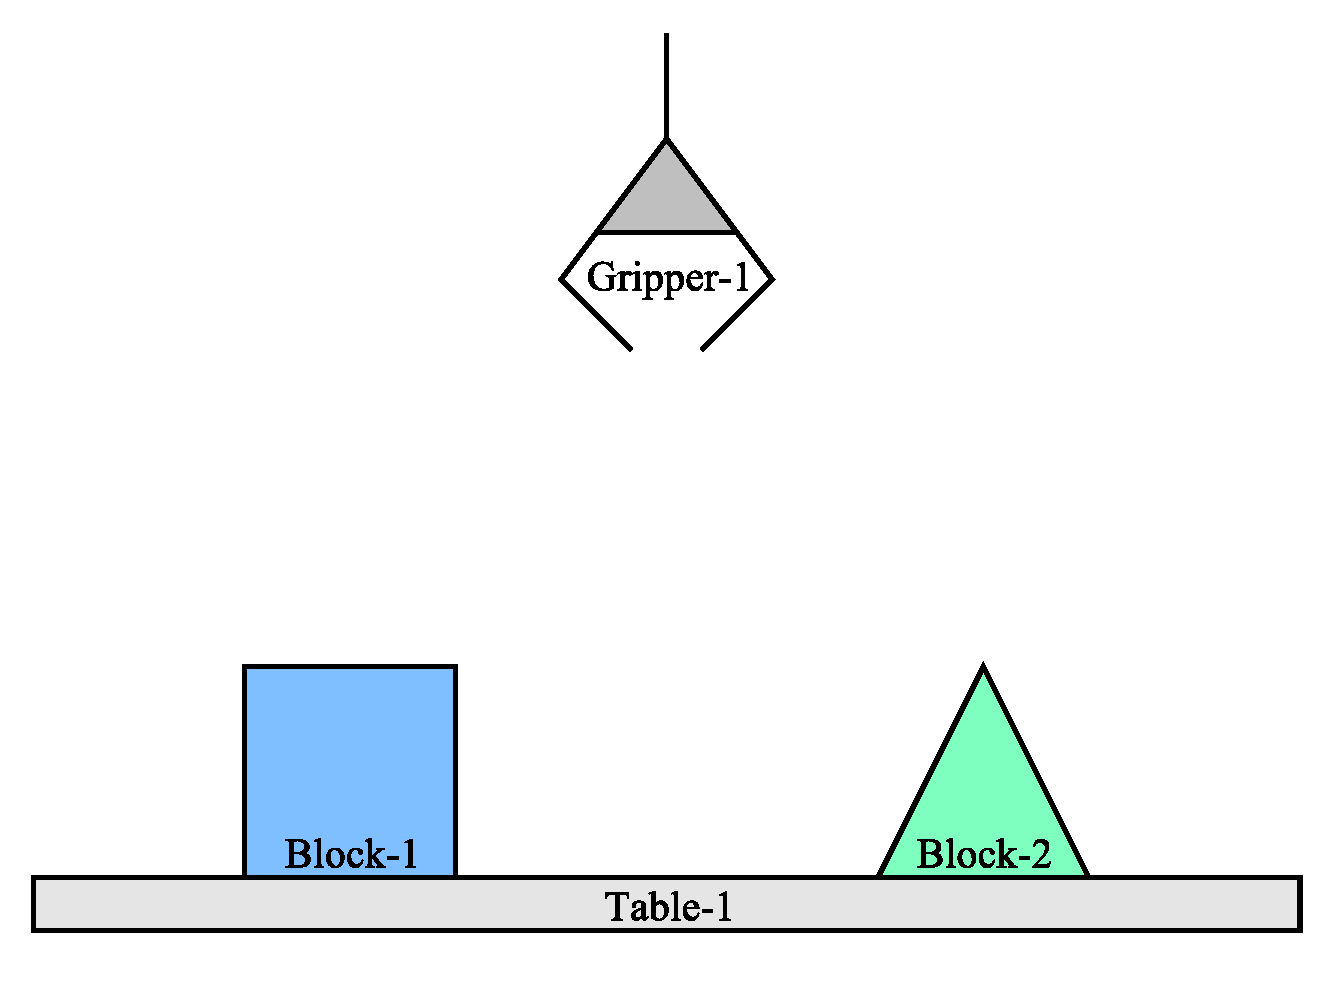
\includegraphics[width=10cm]{gfx/blocks_world_simulation}
\caption{An example for simulation.}
\label{figure:blocks_world_simulation}
\end{figure}

I will begin with a relatively simple model of the activities in
Duration in order to explain the simulation process.  I will explain
the process of simulation before explaining the more detailed
assumptions that I have used in my simulation of the model of mind.
One of the simplest mathematical models is a \emph{set} of symbols.  I
will first describe the simulation model as the mathematical set, $S$,
the state.  Here is an example of a possible symbolization of the
activities shown in \autoref{figure:blocks_world_simulation}:
\begin{equation}
\label{equation:example_initial_state}
S = \left\{
      \begin{array}{l}
        \text{{\tt Block-1-sitting-on-Table-1}}, \\
        \text{{\tt Block-2-sitting-on-Table-1}}, \\
        \text{{\tt Block-1-sitting-on-Table-1}}, \\
        \text{{\tt Gripper-1-being-above-Table-1}}, \\
        \text{{\tt Gripper-1-moving-left}}
      \end{array}
    \right\}
\end{equation}

During the simulation, the state, $S$, changes.  The simulation
process is a discrete stepwise activity that results in different
symbols being contained in the state set, $S$.  I will now describe a
notation for referring to the different states that result from a
simulation process.

\section{Simulation States}

Equations~\ref{equation:simulate_first}
and~\ref{equation:simulate_last} show a notation for referring to the
state of a simulation after a number of simulation steps, $n$.
\begin{align}
\label{equation:simulate_first}
S[0] &= \text{\emph{The Initial State}} \\
\label{equation:simulate_last}
S[n] &= \text{simulate}~S[n-1]
\end{align}
Equation~\ref{equation:simulate_first} defines $S[0]$ to be the
initial representation of the activities in Duration that are being
simulated; an example of the initial state was given previously in
Equation~\ref{equation:example_initial_state}.
Equation~\ref{equation:simulate_last} introduces an explicit reference
to the activity of simulation with the symbol ``simulate.''  Because I
have not yet defined this activity, these equations still have a
reference to the actual dynamic activity of simulation.  I use this
notation to discuss how the state, $S$, changes during the actual
process of simulation.  I will use the notation in
Equation~\ref{equation:simulate_n_steps} to refer to the state of the
simulation after $n$ actual steps of simulation activity:
\begin{equation}
\label{equation:simulate_n_steps}
S[n] = \text{simulate}^n~S[0]
\end{equation}

\section{State Transitions}

\begin{figure}[bth]
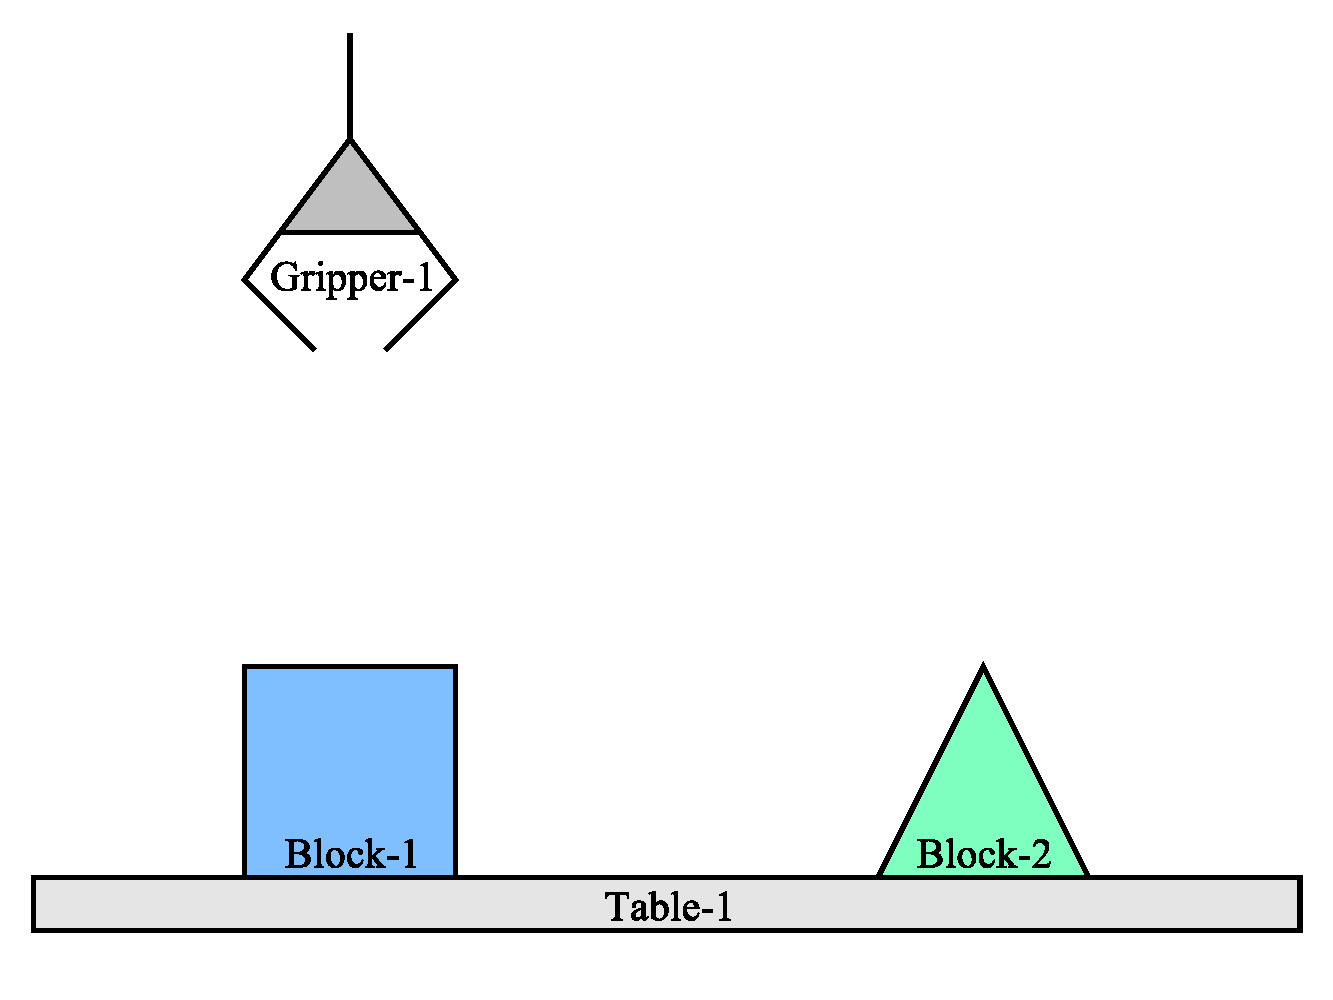
\includegraphics[width=10cm]{gfx/blocks_world_gripper_over_block}
\caption{An example future state of simulation.}
\label{figure:blocks_world_gripper_over_block}
\end{figure}
\autoref{figure:blocks_world_gripper_over_block} shows an example of
the next state of the simulation, $S[1]$.
Equation~\ref{equation:example_next_state} gives an example
description of the next state of the simulation model:
\begin{equation}
\label{equation:example_next_state}
S[1] =
  \left\{
    \begin{array}{l}
      \text{{\tt Block-1-sitting-on-Table-1}}, \\
      \text{{\tt Block-2-sitting-on-Table-1}}, \\
      \text{{\tt Gripper-1-hovering-above-Table-1}}, \\
      \text{{\tt Gripper-1-hovering-above-Block-1}}
    \end{array}
  \right\}
\end{equation}

Now, in order to begin to describe the activity of simulation, we must
explicitly represent the transition, $T$, from one state to another.
I refer to the resulting change to the state of the simulation as a
\emph{state transition}.  The transition, $T[n]$, necessarily consists
two sets that keep track of changes, the \emph{add} set and the
\emph{remove} set, as shown in
Equation~\ref{equation:state_transition}:
\begin{equation}
\label{equation:state_transition}
T[n] = \{T_\text{add}[n], ~T_\text{remove}[n]\}
\end{equation}
Equations~\ref{equation:predictive_state_transition}
through~\ref{equation:transframe_last} give a definition of the
transition, $T[n]$, in terms of the states, $S[n]$ and $S[n+1]$:
\begin{align}
\label{equation:predictive_state_transition}
                    S[n+1] & = S[n] ~{\cup}~ T_\text{add}[n] ~{\setminus}~ T_\text{remove}[n] \\
         T_\text{remove}[n] & ~{\subset}~ S[n] \\
         T_\text{remove}[n] & ~{\not\subset}~ S[n+1] \\
            T_\text{add}[n] & ~{\subset}~ S[n+1] \\
\label{equation:transframe_last}
            T_\text{add}[n] & ~{\not\subset}~ S[n]
\end{align}
Equations~\ref{equation:state_transition_first}
and~\ref{equation:state_transition_last} give the state transition,
$T[n]$, for every step of the simulation:
\begin{align}
  \label{equation:state_transition_first}
     T_\text{add}[n] &= S[n+1] ~{\setminus}~ S[n] \\
  \label{equation:state_transition_last}
  T_\text{remove}[n] &= S[n]   ~{\setminus}~ S[n+1]
\end{align}
Equation~\ref{equation:predictive_state_transition} shows the
predictive potential for knowing the transition, $T[n]$, given the
current state, $S[n]$.


\section{Leftovers...}

\section{Changing states is simulation}

For example, if one writes down the state, $S$, on paper, these
symbols can be perceived and manipulated, creating a new set of
symbols, representing the next state, that can be written down as the
next state.  The activity that changes the current state into the next
state is simulation.

\section{Universal Set}

$\mathcal{S}$

In order to simulate represent the possible symbols that can be
contained within world over time, I use a universal set, $U$.


\section{Examples of Activity in the Physical Layer}

In my English description, I have been careful to not include any
symbols in the physical layer at all; I have used descriptions that
include symbols to refer to example situations, but these example
situations are for the reader's understanding, these example
situations are not included in my model; these are descriptions of the
activity in the physical layer of my model, which does not have
symbols in it.

